\chapter{Early experiments}

\epigraph{And you may ask yourself \\ "Well\dots how did I get here?"}{Once in a Lifetime \\ Talking Heads, 1981}

In this chapter I showcase my journey, experience, pitfalls, breakthroughs, and what led me to working on this thesis, and I will try my best to be open, detailed, celebratory, and critical.

\section{Learning microcontrollers}

I learned how to program microcontrollers around 2010 as an undergraduate student of electrical engineering in Chile using PIC microcontrollers and Microsoft's tools, including the operating system Windows and the C\# programming languages. In parallel, with some classmates we discovered the Arduino Uno microcontroller, and with my friend Braulio we built a robotic guitar tuner, where the Arduino detected the pitch of a string, and made a motor move the tuning gear of the string to match the desired pitch.

\begin{figure}[ht]
  \centering
  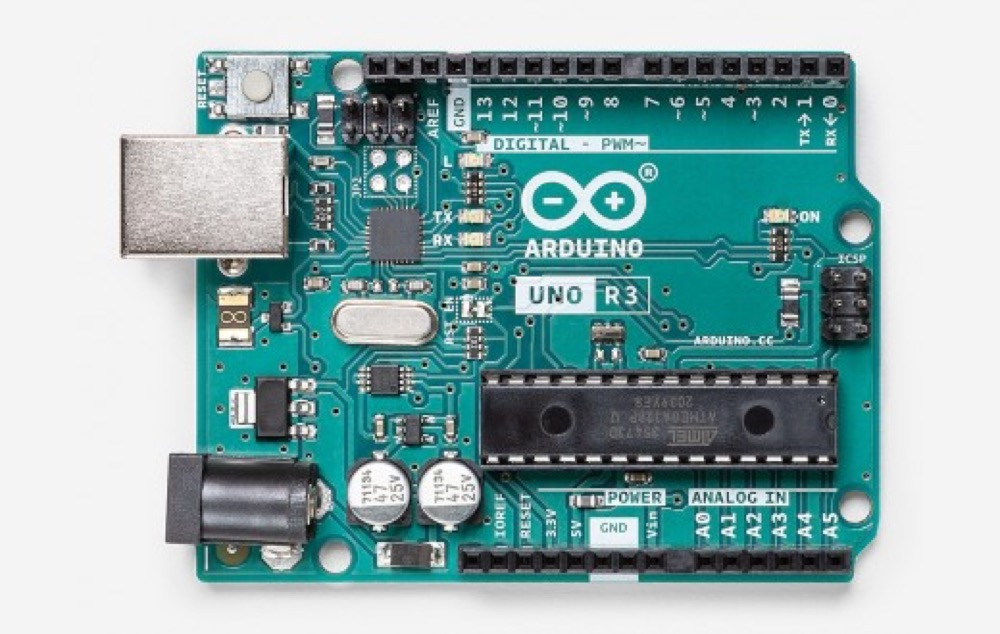
\includegraphics[width=0.75\linewidth,height=0.25\textheight,keepaspectratio]{images/arduino-uno.jpg}
  \caption{Arduino Uno microcontroller}
  \caption*{Retrieved from \cite{website-arduino-uno}}
  \label{fig:arduino-uno}
\end{figure}

Fast forward to 2013, for my thesis I had to complete a capstone project and implement many low-level programming techniques, and Arduinos were not allowed because they were considered a shortcut. With my friend Guillermo we built a robotic device with a PIC microcontroller programmed with C\#. Our code was very specific to that particular chip and project, and hardly reusable or interesting for a wider audience.

I wasn't excited about the prospect of making one-off devices, with non-reusable code that I couldn't share, so I haven't programmed PIC microcontrollers since then. In contrast, Arduinos became a huge part of my practice since then, because of their low cost, ease of programming, and of the available resources and documentation, and user contributed libraries, including the TinyTrainable library developed for this thesis project.

\section{Computer music and physical computing}

During undergrad I took classes and did research with professors and computer musicians Rodrigo Cádiz and Patricio de la Cuadra. With them I learned the fundamentals of computer music, including languages such as Max and Pure Data, which I still use to this day. For a class project I created a spoon synthesizer with masking tape, cardboard, and a Makey Makey, a device created in 2021 by Eric Rosenbaum and Jay Silver from MIT Media Lab's Lifelong Kindergarten research group. This was my introduction to physical computing, as a way of creating custom playful interfaces for manipulating media with computers for arts.
 
\begin{figure}[ht]
  \centering
  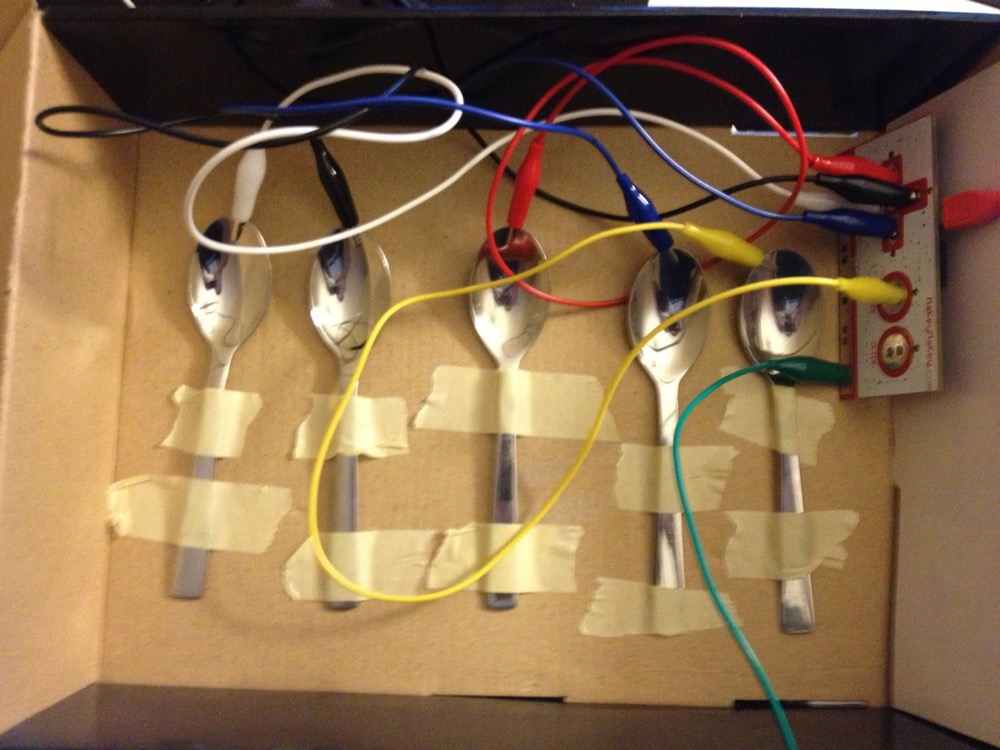
\includegraphics[width=0.75\linewidth,height=0.25\textheight,keepaspectratio]{images/makey-makey-spoons.jpg}
  \caption{Spoons and Makey Makey synthesizer}
  \caption*{Picture taken by myself}
  \label{fig:makey-makey-spoons}
\end{figure}

This was my first time interfacing with my computer without a mouse or a keyboard, but with a flexible instrument that was the result of me tinkering around with cheap reusable materials, in a similar remixable way that I arrange my pedalboards for playing guitar in fleeting ways that are constantly changing.

\section{Learning open source hardware}

After graduation in 2013 I freelanced as a software and technology designer and developer for artists. I learned computer protocols and networks, and wrote custom software for live multimedia theater and music shows. I discovered Processing, a project that Arduino was based on, and I dived deep on computer graphics, interactivity, and it quickly became central to my practice and work.

Realizing that I wanted a bigger community of people to learn media arts with, I researched communities where I thought I could concentrate on learning this craft in a focused and immersive way, so I applied to New York University's Interactive Telecommunications Program (\acrshort{NYU} \acrshort{ITP}), where I joined as a graduate student in 2015. 

In my first semester I took the class Introduction to Physical Computing, taught by one of Arduino's co-creators Tom Igoe. Since I was already familiar with electronics and circuits, I focused on learning interface design, human computer interaction, open source hardware and software, and physical computing education.

During my research I was introduced to a wider ecosystem of microcontrollers beyond Arduino, that were possible because of its open source nature and the community behind it. My favorite example is the Teensy by PJRC, which captivated me by its USB MIDI capabilities, which allowed for standalone \acrshort{MIDI} operation, and the creation of plug and play devices that needed no additional setup or scripting. Also by its audio library, which allowed me to create interactive standalone experiences, playing audio samples and applying audio effects.

\begin{figure}[ht]
  \centering
  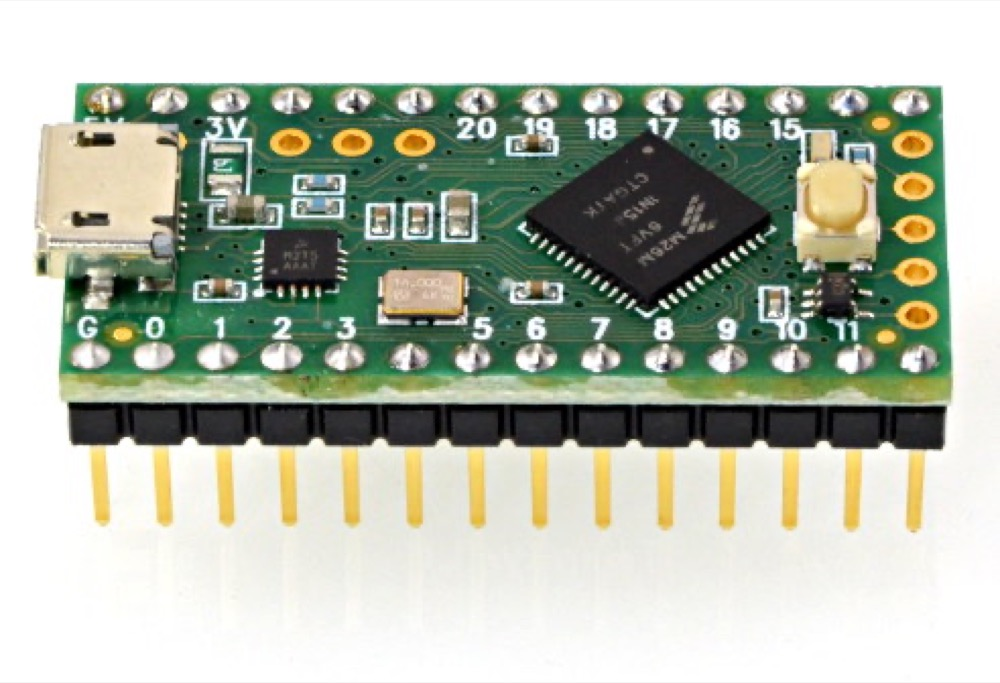
\includegraphics[width=0.75\linewidth,height=0.25\textheight,keepaspectratio]{images/pjrc-teensy-lc-with-pins.jpg}
  \caption{PJRC Teensy LC microcontroller with pins}
  \caption*{Retrieved from \cite{website-pjrc-teensy-lc-with-pins}}
  \label{fig:pjrc-teensy-lc-with-pins}
\end{figure}

\section{Processing and p5.js}

The program at \acrshort{NYU} \acrshort{ITP} is by definition in constant change, and I feel lucky because in my first semester's Introduction to Computational Media class we were taught p5.js instead of Processing, a change that hadn't happened in a year. I had almost no experience in web programming, and I mostly didn't see the point of it.

Lauren McCarthy, the creator of the p5.js library, was a professor at \acrshort{NYU} in my first year, and I took her class Performing User, about performance art and technology, and it was my favorite class in graduate school.

At \acrshort{NYU} \acrshort{ITP} I but mostly about web and scripting, and my thesis concentrated on open source, performance art, with only a small hardware component in the form of a Raspberry Pi computer with a countdown timer to my projected death time, according to data by the United Nations, based on my assigned-at-birth-gender and my birth place.

\section{Teaching}

After graduating from \acrshort{NYU} \acrshort{ITP} I focused on media arts education, writing tutorials, teaching introduction to programming workshops for artists.

When I joined MIT Media Lab in 2019, I made the conscious decision of focusing on hardware, to give my creations a life outside of my computer, also inspired by newer restrictive developments by Apple, such as restricting the use of apps created by unregistered developers. In my first semester, which ended up being the only on-campus semester I had, I was introduced by my friend Will Freudenheim to the Shbobo synthesizers by Peter Blasser.

\section{Publishing on the web}

\section{Publishing libraries}

I was partially aware of the instruments made by Peter Blasser, in particular the analog ones.

While at MIT Media Lab, I was delighted by the newer versions of Teensy, which are even faster and more powerful, and which led me to start designing handheld samplers for field recordings, and other standalone devices.

This in turn led me to review the current \acrshort{NYU} \acrshort{ITP} materials for physical computing, where they currently stopped using the now classic Arduino Uno, and have incorporated in their teaching the new series of Arduino Nano microcontrollers, which I based my thesis on.

In particular, the Arduino Nano 33 \acrshort{BLE} Sense I am using, comes with 9 sensors, to measure and detect acceleration, movement, distance, color, and a microphone. This is an amazing breakthrough, since now we can use all this data without having to purchase, install, or calibrate the sensors.

I am using the Arduino's sensors to gather multimedia input data, analyze it with \acrshort{ML}, and then respond with multimedia outputs.

\section{Artistic ML}

My first experiment in this field was with my \acrshort{NYU} \acrshort{ITP} classmate Corbin Ordel, who was a student at Gene Kogan's \acrshort{ML} for Artist class. Together we audited Rebecca Fiebrink's \acrshort{ML} for Musicians and Artists class, available at the Kadenze platform, and learned the Wekinator platform.

Our project is Piano Die Hard, a digital sculpture consisting on a piano that reacted in real time, 


teamed up to hack a project we called Piano Die Hard, built with open source tools such as Wekinator, Arduino, openFrameworks, and using the \acrshort{ML} algorithm KNN. We created a video database of explosions in the Die Hard movie franchise, and another one of other 1980's movies with no explosions, and we trained our \acrshort{ML} algorithm to distinguish between the categories explosion and no explosion. We featured this project at a \acrshort{NYU} \acrshort{ITP} show, were written up at the Daily Beast newspaper, and exhibited our work at the alt-ai conference.

In 2017, while I was finishing my appointment as research resident at \acrshort{NYU} ITP, Cristóbal Valenzuela had started the project RunwayML as his master's thesis, which is now a company led by Cristóbal, Alejandro Matamala and Anastasis Germanidis.

At \acrshort{NYU} \acrshort{ITP} I also saw the first experiments with deeplearn.js, later TensorFlow.js, which soon became the foundation of the ml5.js library, a wrapper for TensorFlow.js, for on-the-browser \acrshort{ML}.

I decided I wanted to dip my toes in \acrshort{ML}, so I took a month-long intensive class at the School of Machines in Berlin, Germany, facilitated by Gene Kogan and Andreas Refsgaard, and organized by Rachel Uwa.


A big inspiration for this thesis has been the book on GANs by Casey Reas, published by Anteism, as of 2021 on its second edition. It’s an arts-first book that contextualizes the use of \acrshort{ML} algorithms for the creation of images, and uses the metaphor of these algorithms as being similar to the development of the camera. Artists don’t need to understand all the physics or mechanics behind a camera in order to make art with it, but it can help to understand it too. I think \acrshort{ML} is also a game changer for instrument making, and \acrshort{ML} introduces new civic complexities, and my thesis tries to follow the example of this book, to introduce the technology and contextualize for a new generation of artists and instrument makers.

Since many \acrshort{ML} projects rely on proprietary hardware, such as NVIDIA GPUs, or rely on the cloud for faster compilation times, for this thesis I decided to make open source \acrshort{ML} projects that people could read and understand and remix and hack.

TODO: mention the impact of the documentary Coded Bias, and how these researchers impacted my desire to make my thesis. Also mention how right before pandemic I had started a pottery class, with the intention of making clay-based instruments for thesis, as a metaphor of making code and hardware and software feel fluid and not static, I want to empower people to program, in particular \acrshort{ML} because of its dangerous implementations by oppressive governments and corporations, and in particular for arts, for making artists dream come true.
